\section{Métodos y condiciones de los experimentos}

Realizamos capturas de paquetes en distintos horarios en la red LAN hogareña de cada integrante de este trabajo, con el objetivo de obtener un muestreo diverso. Utilizamos la herramienta Wireshark para capturar los paquetes de las redes, que luego exportamos a archivos .csv y .pcap para analizarlos con Pandas. Extendimos el código \texttt{Python} provisto para que tome como fuente un archivo .pcap en lugar de capturar la red en tiempo real, calcule la frecuencia e información de cada símbolo y la entropía de las fuentes y luego escriba los resultados en archivos .csv para estudiarlos.

\begin{table}[H]
    \begin{center}
        \begin{tabular}{||c c c c c c||} 
             \hline
             Dataset & Tecnología & Tamaño de la red & Tamaño de la muestra & Hora & Día \\ [0.5ex] 
             \hline\hline
             $Red 1$ & Wi-Fi & Red LAN & 39511 tramas & 15:20hs & Viernes \\ 
             \hline
             $Red 2$ & Wi-Fi & Red LAN & 23841 tramas & 16hs & Sábado \\
             \hline
             $Red 3$ & Wi-Fi & Red LAN & 50695 tramas & 19:40hs & Viernes \\ [1ex] 
             \hline
        \end{tabular}
    \end{center}
    \caption{Características de las capturas}
    \label{tab: condiciones de datasets}
\end{table}


\subsection{Contexto de las capturas} 

\begin{description}
    \item[Hogar del integrante 1 (dataset \emph{Red1}):] En el momento del análisis, había una computadora y un celular conectados a la red wifi. Se capturaron paquetes durante una hora, haciendo un uso de multimedia sobre la red. Se obtuvieron 39511 tramas. 
    
    \item[Hogar del integrante 2 (dataset \emph{Red2}):] Se capturaron paquetes durante una hora desde una computadora portatil conectada a una red wifi doméstica con acceso a Internet, en la que además se hallaban conectados dos celulares, una tablet, dos cámaras de seguridad y dos televisores. Dentro del transcurso de la captura, se ejecutó una aplicación que determina los dispositivos que están conectados a una red wi-fi y, como se desarrolla más adelante, esto tuvo un efecto en los resultados obtenidos.
    
    \item[Hogar del integrante 3 (dataset \emph{Red3}):] Desde una computadora portatil, se capturaron paquetes durante una hora en una red doméstica. En esta red estaban ademas conectados: Una computadora de escritorio por ethernet, dos celulares y un repetidor de wi-fi al que estaban probablemente conectadas una tablet y una computadora portatil.

\end{description}

\subsection{Explicación del código}
\subsubsection{Análisis 1 - Fuente $S_{1}$}
Tomando como base el código dado por la cátedra, restaba agregar funciones que se encarguen de calcular la frecuencia e información de cada símbolo, la entropía de la fuente y el porcentaje de tráfico \texttt{Broadcast} vs \texttt{Unicast}.

Habiendo procesado los paquetes de cada muestra, obtuvimos un diccionario donde los símbolos eran las claves y el valor era la cantidad de apariciones durante el análisis. Para calcular la frecuencia de cada símbolo iteramos por las claves del diccionario y calculamos su porcentaje de apariciones frente a todos los paquetes.

Para calcular la información de cada símbolo, calculamos el logaritmo base 2 de la frecuencia de cada uno (calculado previamente) y lo negamos.
 
Finalmente, dado que nuestra fuente no es equiprobable, calculamos la \texttt{entropía} como la suma de la multiplicación de la información que provee cada símbolo y su frecuencia.
\begin{equation} \label{eq24}
\begin{split}
H(S) = {\sum_{s \in S}frecuencia_{s} * informacion_{s}}
\end{split}
\end{equation}

Respecto del cálculo del porcentaje de tráficco \texttt{Broadcast} vs \texttt{Unicast}, lo que hicimos fue contar sus apariciones durante el análisis de las muestras.

\subsubsection{Análisis 2 - Fuente $S_{2}$}
Dado que necesitamos distinguir los hosts de paquetes \texttt{ARP} que habían aparecido durante las mediciones de cada muestreo, decidimos utilizar como símbolo la dirección \texttt{IP} origen de la trama. Este valor se encuentra en el atributo \texttt{psrc} de los paquetes \texttt{ARP}. Como se muestra en la Figura~\ref{code: callback_2} tomamos las direcciones \texttt{IP} origen de cada paquete recibido y aumentamos el contador correspondiente en el diccionario S2 obteniendo al finalizar la cantidad total de apariciones de cada una.

Los calculos de la información y frecuencia por símbolo, así como también entropía se hace de forma análoga al análisis 1.

\begin{figure}[H]
    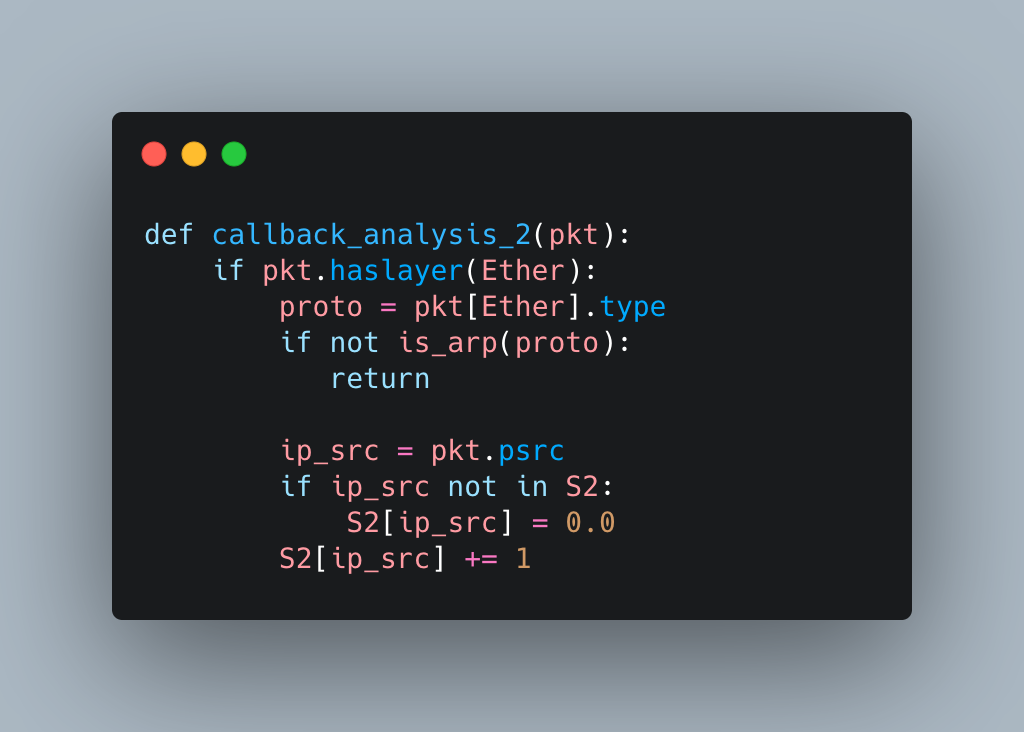
\includegraphics[width=0.7\textwidth]{images/resultados_generales/codigo_analisis_2.png}\vspace{1em}
    \centering
    \caption{Función ejecutada al procesar cada trama de la muestra}
    \label{code: callback_2}
\end{figure}

\subsection{Justificación de elección de la fuente $S_{2}$} 
Como mencionamos previamente, con el objetivo de distinguir hosts de nuestra red definimos como símbolos a las direcciones \texttt{IP} origen de las tramas. Esta elección nos resultó natural debido a que, si un dispositivo se encuentra en una red, es altamente probable que en algún momento envíe un paquete y no solo se dedique a recibir.

Otra opción que tuvimos en cuenta fue tomar como símbolos las direcciones \texttt{IP} destino de las tramas, aunque rápdiamente notamos que podrían aparecer tramas con destinos inexistentes en la red, por lo que no era una opción viable. Luego pudimos comprobar que éste efectivamente era un caso posible: durante el análisis del comportamiento de las redes presentadas en el trabajo, notamos cómo algunas aplicaciones hacian uso de técnicas de fuerza bruta para, por ejemplo, encontrar los hosts activos en la red. Esto generaba muchas tramas donde la dirección \texttt{IP} destino no era un nodo válido dentro de la red.

